%%
%% This is file `sample-sigconf.tex',
%% generated with the docstrip utility.
%%
%% The original source files were:
%%
%% samples.dtx  (with options: `sigconf')
%% 
%% IMPORTANT NOTICE:
%% 
%% For the copyright see the source file.
%% 
%% Any modified versions of this file must be renamed
%% with new filenames distinct from sample-sigconf.tex.
%% 
%% For distribution of the original source see the terms
%% for copying and modification in the file samples.dtx.
%% 
%% This generated file may be distributed as long as the
%% original source files, as listed above, are part of the
%% same distribution. (The sources need not necessarily be
%% in the same archive or directory.)
%%
%%
%% Commands for TeXCount
%TC:macro \cite [option:text,text]
%TC:macro \citep [option:text,text]
%TC:macro \citet [option:text,text]
%TC:envir table 0 1
%TC:envir table* 0 1
%TC:envir tabular [ignore] word
%TC:envir displaymath 0 word
%TC:envir math 0 word
%TC:envir comment 0 0
%%
%%
%% The first command in your LaTeX source must be the \documentclass
%% command.
%%
%% For submission and review of your manuscript please change the
%% command to \documentclass[manuscript, screen, review]{acmart}.
%%
%% When submitting camera ready or to TAPS, please change the command
%% to \documentclass[sigconf]{acmart} or whichever template is required
%% for your publication.
%%
%%
\documentclass[sigconf]{acmart}

%%
%% \BibTeX command to typeset BibTeX logo in the docs
\AtBeginDocument{%
  \providecommand\BibTeX{{%
    Bib\TeX}}}

%% Rights management information.  This information is sent to you
%% when you complete the rights form.  These commands have SAMPLE
%% values in them; it is your responsibility as an author to replace
%% the commands and values with those provided to you when you
%% complete the rights form.
\setcopyright{acmcopyright}
\copyrightyear{2018}
\acmYear{2018}
\acmDOI{XXXXXXX.XXXXXXX}

%% These commands are for a PROCEEDINGS abstract or paper.
\acmConference[Conference acronym 'XX]{Make sure to enter the correct
  conference title from your rights confirmation emai}{June 03--05,
  2018}{Woodstock, NY}
%%
%%  Uncomment \acmBooktitle if the title of the proceedings is different
%%  from ``Proceedings of ...''!
%%
%%\acmBooktitle{Woodstock '18: ACM Symposium on Neural Gaze Detection,
%%  June 03--05, 2018, Woodstock, NY}
\acmPrice{15.00}
\acmISBN{978-1-4503-XXXX-X/18/06}


%%
%% Submission ID.
%% Use this when submitting an article to a sponsored event. You'll
%% receive a unique submission ID from the organizers
%% of the event, and this ID should be used as the parameter to this command.
%%\acmSubmissionID{123-A56-BU3}

%%
%% For managing citations, it is recommended to use bibliography
%% files in BibTeX format.
%%
%% You can then either use BibTeX with the ACM-Reference-Format style,
%% or BibLaTeX with the acmnumeric or acmauthoryear sytles, that include
%% support for advanced citation of software artefact from the
%% biblatex-software package, also separately available on CTAN.
%%
%% Look at the sample-*-biblatex.tex files for templates showcasing
%% the biblatex styles.
%%

%%
%% The majority of ACM publications use numbered citations and
%% references.  The command \citestyle{authoryear} switches to the
%% "author year" style.
%%
%% If you are preparing content for an event
%% sponsored by ACM SIGGRAPH, you must use the "author year" style of
%% citations and references.
%% Uncommenting
%% the next command will enable that style.
%%\citestyle{acmauthoryear}


%%
%% end of the preamble, start of the body of the document source.
\begin{document}

%%
%% The "title" command has an optional parameter,
%% allowing the author to define a "short title" to be used in page headers.
\title{CS527 midterm report}

%%
%% The "author" command and its associated commands are used to define
%% the authors and their affiliations.
%% Of note is the shared affiliation of the first two authors, and the
%% "authornote" and "authornotemark" commands
%% used to denote shared contribution to the research.
\author{Yiteng Hu}
\authornote{Both authors contributed equally to this research.}
\email{yitengh2@illinois.edu}
\author{Yuehao Shi}
\authornotemark[1]
\email{yuehaos2@illinois.edu}
\affiliation{%
  \institution{UIUC}
  \city{Champaign}
  \state{IL}
  \country{USA}
  \postcode{61801}
}

%%
%% By default, the full list of authors will be used in the page
%% headers. Often, this list is too long, and will overlap
%% other information printed in the page headers. This command allows
%% the author to define a more concise list
%% of authors' names for this purpose.
\renewcommand{\shortauthors}{Trovato et al.}

%%
%% The abstract is a short summary of the work to be presented in the
%% article.
\begin{abstract}
  The article presents an extension of the FreeFuzz automated fuzz testing tool to test PaddlePaddle, 
  an emerging open-source deep learning library. The team aims to improve the reliability of deep learning 
  libraries by identifying and fixing potential bugs and vulnerabilities. The proposed solution involves 
  four steps: code collection, instrumentation, mutation test, and oracle test. The team has completed 
  the code collection and instrumentation stages, while the mutation stage is yet to be completed. 
  The team has encountered challenges due to different installation settings and environments for
   TensorFlow and PaddlePaddle packages and insufficient data collection, delaying the mutation strategy development.
    The team plans to use metrics such as covered APIs, the size of the value space, and line coverage to evaluate the effectiveness 
    of the Freefuzz tests for PaddlePaddle and compare them to other state-of-the-art deep learning library testing techniques.
\end{abstract}

%%
%% The code below is generated by the tool at http://dl.acm.org/ccs.cfm.
%% Please copy and paste the code instead of the example below.
%%

%%
%% Keywords. The author(s) should pick words that accurately describe
%% the work being presented. Separate the keywords with commas.
\keywords{Fuzz testing, Deep learning libraries, PaddlePaddle, Automated testing, Mutation testing}
%% A "teaser" image appears between the author and affiliation
%% information and the body of the document, and typically spans the
%% page.


%%
%% This command processes the author and affiliation and title
%% information and builds the first part of the formatted document.
\maketitle

\section{problem}
\par Deep learning (DL) has become an indispensable tool for solving complex problems in various domains, including computer vision, natural language processing, and speech recognition. DL libraries, such as TensorFlow and PyTorch, are essential tools for building, optimizing, and running DL models. However, testing these libraries can be challenging due to their complexity and the lack of effective testing techniques.
\par Testing DL systems is challenging because they typically comprise multiple layers of neural networks that perform intricate computations on large amounts of data. These computations involve non-linear transformations that are often difficult to reason about. Additionally, DL systems are commonly trained on vast datasets that are challenging to reproduce, adding to the complexity of testing.
\par To address these challenges, researchers have proposed various techniques for testing DL systems, including mutation testing, adversarial testing, differential testing, and fuzzing. Fuzzing is a testing technique that involves generating random inputs to test software systems. It has been successfully applied to various types of software systems, including web applications, operating systems, and compilers.
\par FreeFuzz is a recent approach that utilizes open source mining to fuzz DL libraries. This automated fuzz testing tool has been effectively employed to test TensorFlow and PyTorch libraries by generating a large number of test cases from code snippets in library documentation, developer tests, and DL models in the wild. FreeFuzz uses a line coverage metric to measure its code coverage.
\par However, testing the emerging open-source deep learning library, PaddlePaddle, using automated techniques like FreeFuzz presents challenges due to the complexity of its public APIs, which are mainly exposed in Python. The dynamic typing used in these APIs makes it challenging to automatically determine the API input parameter types. Furthermore, PaddlePaddle library has unique features and functionalities that require specific testing techniques, making it necessary to extend FreeFuzz to test this library.
\par The project team aims to extend the existing fuzzing system to test PaddlePaddle library. The goal is to improve the reliability of these libraries by discovering and fixing potential bugs and vulnerabilities. The significance of this research lies in the fact that DL libraries play a crucial role in our daily lives, but bugs in these systems can have disastrous consequences. Surprisingly, despite the importance of DL library reliability, there is only limited work for testing DL libraries. One example of this is CRADLE, which uses pre-existing DL models to test Keras and its backends, and addresses the issue of test oracles through differential testing. To expand on this approach, LEMON enhances CRADLE by utilizing various model mutation rules to create a wider range of DL models. This enables the invocation of more library code and exposes a greater number of potential bugs in the DL library.
\par In conclusion, while DL systems are complex and challenging to test using conventional techniques, fuzzing has emerged as a promising approach to testing DL libraries. FreeFuzz has been effectively used to test TensorFlow and PyTorch libraries, and extending it to test PaddlePaddle library will further enhance the reliability of DL libraries. This research contributes to improving the quality of DL libraries and reducing the likelihood of disastrous consequences caused by bugs in these systems.



\section{solution}
\par To address the challenge of testing PaddlePaddle library using automated techniques like FreeFuzz, we propose extending FreeFuzz to test PaddlePaddle library using the same method mentioned in the FreeFuzz paper. More specifically, we will obtain code/models from three different sources: 1) code snippets from the library documentation, 2) library developer tests, and 3) DL models in the wild. By combining these three sources of input, we can generate a large number of test cases that cover different parts of the PaddlePaddle library.
\par To address the challenge of dynamic typing in Python, we will use type annotations to specify the input parameter types for each API. Type annotations provide a way to specify the expected types of function arguments and return values in Python [15]. By using type annotations, we can automatically determine the API input parameter types and generate valid test cases.
\par We will use the same line coverage metric used in the FreeFuzz paper to measure our code coverage. This metric measures the percentage of lines of code executed during testing. We will also evaluate our approach on a set of benchmark programs that use PaddlePaddle library as their backend engine.
\par In conclusion, extending FreeFuzz to test PaddlePaddle library is an important step towards improving the quality and reliability of DL libraries. By using the same method mentioned in the FreeFuzz paper and incorporating type annotations for dynamic typing in Python, we can generate effective tests for PaddlePaddle library and improve its robustness and correctness. Furthermore, our approach can help identify and fix bugs in PaddlePaddle library, which can lead to better performance and accuracy of DL models built using this library. Our approach can also be extended to test other DL libraries that are mainly exposed in Python and have dynamic typing.
\par Overall, our proposed approach can significantly improve the testing of DL libraries and help ensure their correctness and reliability. By generating a large number of test cases that cover different parts of the library, we can increase the code coverage and identify potential bugs or issues. This can ultimately lead to better quality DL models and more reliable applications built using these models.

  \begin{figure}[h]
    \centering
    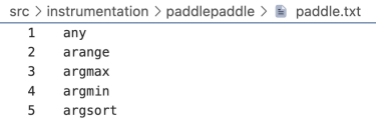
\includegraphics[width=\linewidth]{1.png}
    \caption{Work flow of Freefuzz}
  \end{figure}
  \subsection{Code Collection}
  \par The methodology for collecting code snippets for the PaddlePaddle framework was inspired by the FreeFuzz research paper. 
  The team obtained code snippets from three primary sources, namely: (1) code snippets from the official documentation, 
  (2) testing files from the PaddlePaddle library developer tests, and (3) deep learning models in the wild. 
  The team also collected API executions of PaddlePaddle based on the same three sources.

  \par The official website of PaddlePaddle was the primary source of code snippets, which provided all available API names, 
  definitions, and execution examples for the latest version of the framework. To automate the process of parsing the documentation and obtaining the code snippets, 
  the team utilized the bs4 Python package. 

  \par The team also collected testing files from the PaddlePaddle library developer tests. 
  There are a total of 692 testing files in the latest version of PaddlePaddle, which the team obtained by cloning the latest PaddlePaddle official repository into their local machine.

  \par Lastly, the team obtained code from deep learning models in the wild. 
  The team collected publicly available PaddlePaddle models and utilized them as a source of real-world use cases for testing the PaddlePaddle libraries. 
  For instance, the PaddleNLP package, which is an easy-to-use and powerful NLP library that leverages PaddlePaddle as a basic structure, provided numerous Paddle API calls that were suitable for collecting APIs for fuzzing. 
  The team executed all testing files for this package to augment their API pool with this package.
    
  \subsection{instrumentation}
  \par The second stage of the Freefuzz adaptation process for PaddlePaddle involves dynamic tracing with instrumentation, 
  which allows Freefuzz to intercept selected PaddlePaddle APIs and collect information about their execution, 
  including input argument values and output values. This information is stored in MongoDB in JSON format to create the necessary type space, 
  API value space, and argument value space for later fuzzing stages.


  
  \begin{figure}[h]
    \centering
    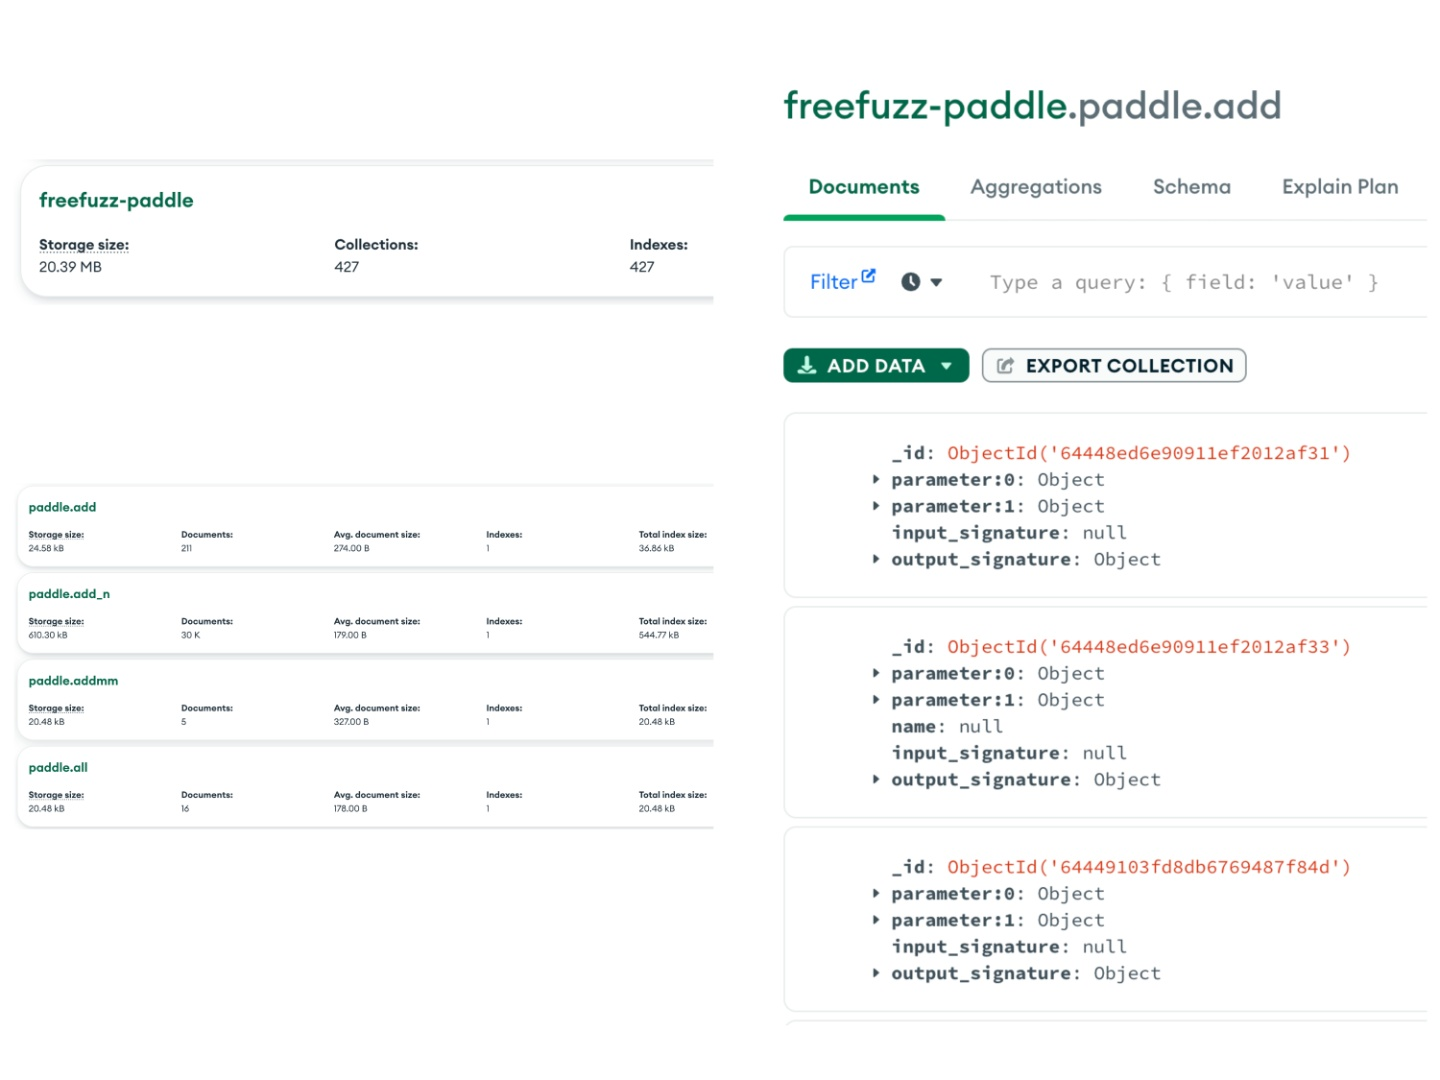
\includegraphics[width=\linewidth]{3.png}
    \caption{Database overview (left top), Database collections (left bottom), and Collection detail (right)}
  \end{figure}
  
  \subsection{Mutation Test}

  In this phase, We applies various mutation rules to mutate the arguments.\cite{w1}
  \newline \textbf{Mutation Rules}. The mutation rules for FreeFuzz are composed
  of two parts: type mutation and value mutation, shown in Tables 1
  and 2, respectively. Type mutation strategies include Tensor Dim
  Mutation that mutates n1-dimensional tensors to n2-dimensional
  tensors, Tensor Dtype Mutation that mutates the data types of tensors without changing their shapes, Primitive Mutation that mutates
  one primitive type into another, as well as Tuple Mutation and List
  Mutation that mutate the types of elements in collections of heterogeneous objects.\cite{w1}
  \newline Different from pytorch and tensorflow, paddle doesn't have the api to generate random complex values. Thus, the team
  created such function which is randomizing the real part and imaginary part of complex number respectively.
 
  \begin{table}[h]
    \centering
    \caption{Type Mutation}
    \label{tab:freq}
    \begin{tabular}{ccl}
      \toprule
      Mutation Strategies&$T_1$&$T_2$\\
      \midrule
      Tensor Dim Mutation & tensor<n1,DT>& tensor<n2,DT>\\
      Tensor Dtype Mutation & tensor<n,$DT_1$>& tensor<n,$DT_2$>\\
      Primitive Mutation & $T_1$ = int|bool|float|str & $T_2$\\
      Tuple Mutation & $(T_i ^ {i\in 1...n})$&$(typemutate(T_i ^ {i\in 1...n}))$ \\
      List Mutation & $[T_i ^ {i\in 1...n}]$&$[typemutate(T_i ^ {i\in 1...n})]$ \\
    \bottomrule
  \end{tabular}
  \end{table}

  \begin{table}[h]
    \centering
    \caption{Value Mutation}
    \label{tab:freq}
    \begin{tabular}{ccl}
      \toprule
      Mutation Strategies&$T$&$V$\\
      \midrule
      Random Tensor Shape& tensor<n,DT>& tensor(shape=[randint()],dtype=DT)\\
      Random Tensor Value& v: tensor<n,DT>& tensor(shape=v.shape,dtype=DT).rand()\\
      Random Primitive& int|bool|float|str & rand(int|bool|float|str)\\
      Random Complex& real + imag & rand(real) + rand(imag)\\
      Random Tuple& $(T_i ^ {i\in 1...n})$&$(value\_mutate(T_i ^ {i\in 1...n}))$ \\
      Random List& $[T_i ^ {i\in 1...n}]$&$[value\_mutate(T_i ^ {i\in 1...n})]$ \\
    \bottomrule
  \end{tabular}
  \end{table}


  We collected different types for PaddlePaddle, which are shown in the figure3. 
  And we decide to extend the mutation strategies used in the original paper.
  To summarize, the team has selected a subset of APIs as a proof of concept to 
  demonstrate the feasibility of applying the complete Freefuzz testing process to the PaddlePaddle package, 
  as set out in the midterm goals.
  \begin{figure}[h]
    \centering
    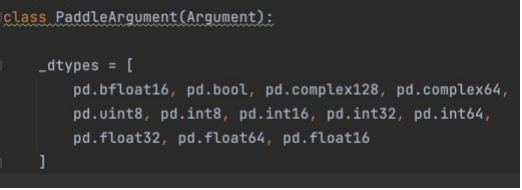
\includegraphics[width=\linewidth]{4.png}
    \caption{data types in PaddlePaddle}
  \end{figure}


  \subsection{Test Oracle}


\section{Evaluation}
  \subsection{Implementation}
  \textbf{Code Collection}. For code collected from Paddle official documentation, 
  the resulting scripts and outputs for crawling can be accessed from the $/src/reptile directory$, 
  while the API execution code snippets are available in \verb|src/reptile/code_snippets|. 
  After filtering out invalid results from the reptile tool and several API execution codes that caused instrumentation to crash, 
  the team obtained a total of 826 API names, 720 API definitions, and 1493 executable code snippets from the official PaddlePaddle documentation website.
  \par For official test source, the team cloned Paddle source code from Github and executed all \verb|test_*.py| files in Paddle/test folder using pytest as automation testing tool. 
  After removing unsupported imports by removing invalid tests, there are 2741 tests left. After executing all 2741 tests, only one more collection shown on MongoDB, 
  but the total size in database increased  \verb|2%|, indicating significant API execution overlap between official documentation code snippets and testing documents.
  For wild Paddle project source, the team collected PaddleNLP package and ran testing files inside it.
  
  \begin{figure}[h]
    \centering
    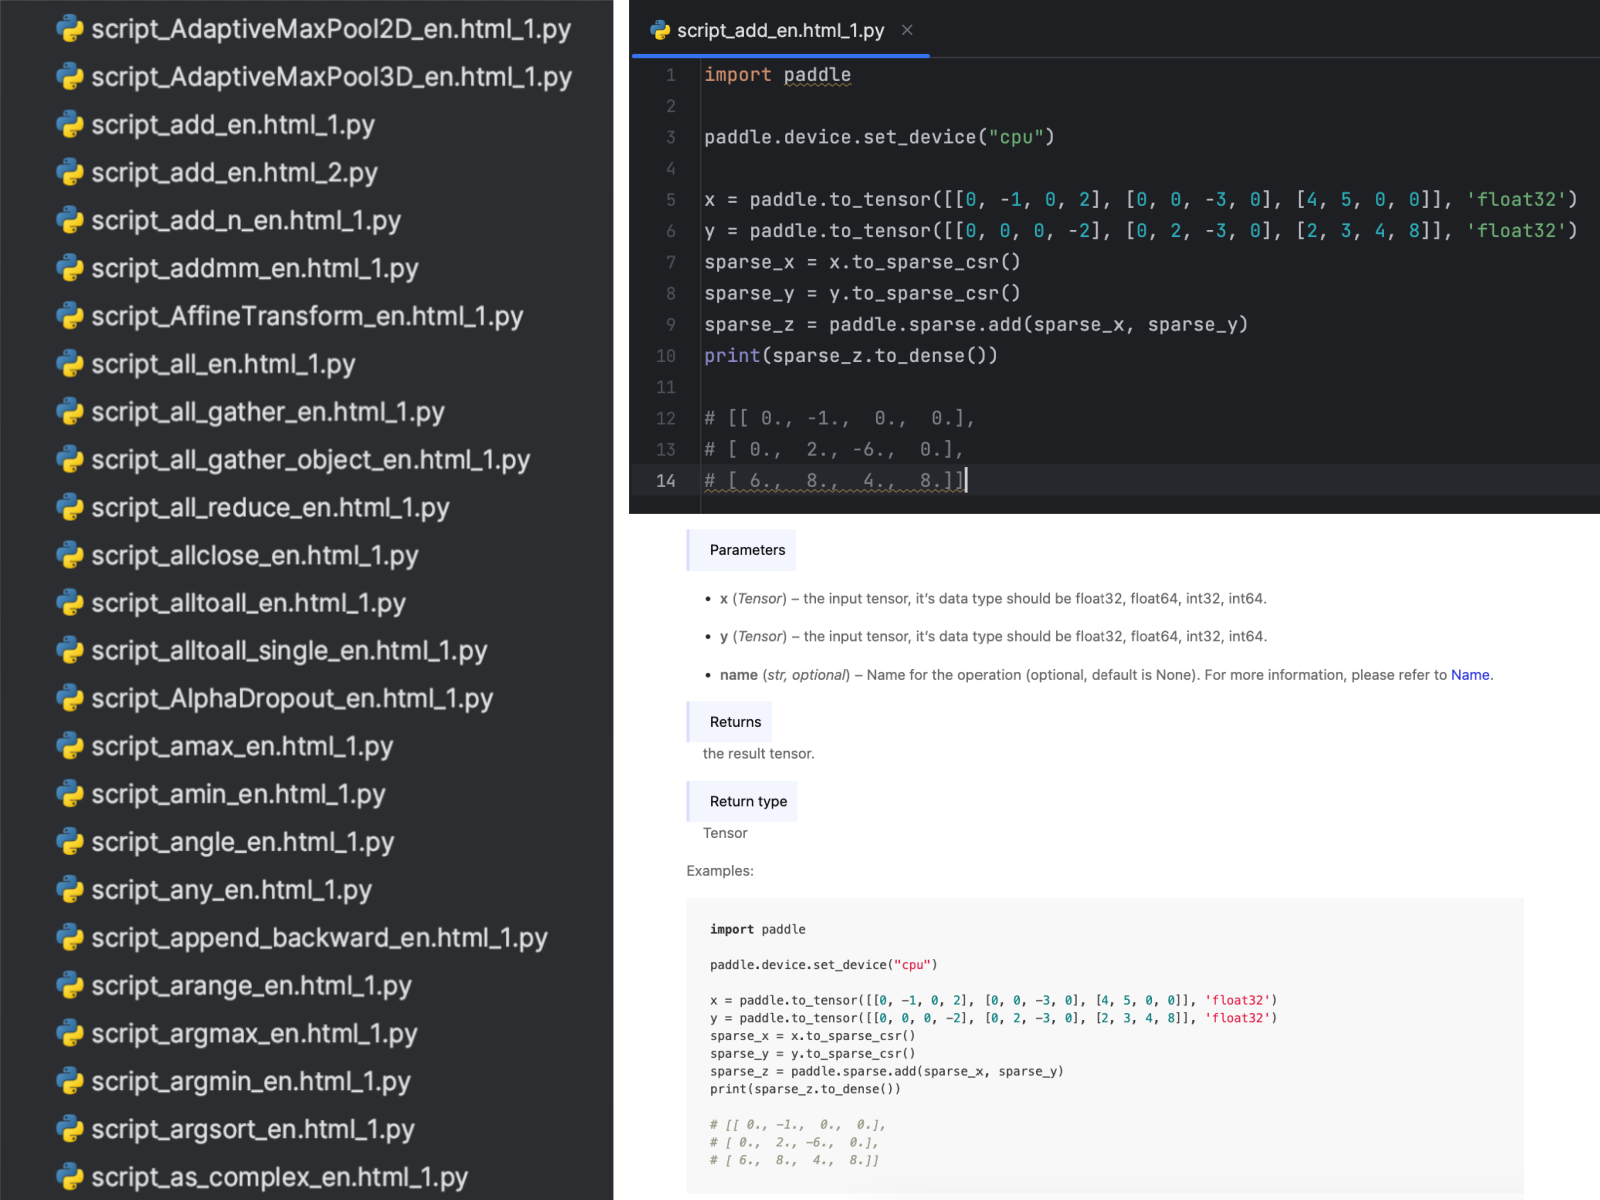
\includegraphics[width=\linewidth]{2.png}
    \caption{Code snippets list (left), code snippet detail (right top), and code snippet origin (right bottom)}
  \end{figure}  

  \textbf{Instrumentation}. To implement this instrumentation stage, the team repurposed the code used for testing the PyTorch library, 
  utilizing functions such as \verb| hijack|, \verb| decorate_class|, \verb| decorate_function|, and \verb| write_fn|. Different sources of code collection require different ways of implementing instrumentation. 
  During the process, the team found that not all collected APIs are valid for instrumentation, and decided to focus on fuzzing Paddle functions, keeping 511 APIs over 720 defined APIs on the Paddle official website.
  
  \par For the code collected from the official documentation, the team executed all 1493 code snippets, but several code snippets could not compile during instrumentation due to typo errors on the Paddle official documentation examples. 
  After executing all code snippets and hijacking API execution information into MongoDB, there are a total of 420 collections in MongoDB after running all code snippets, 
  where one collection means the execution information of one API. Over 511 selected Paddle APIs, 420 APIs get executed and stored, so official documentation code snippets contributed \verb|82%| of targeted API.

  \par For the official test code, the team cloned Paddle source code from Github and executed all \verb|test_*.py| files in Paddle/test folder using pytest as automation testing tool. 
  After removing unsupported imports by removing invalid tests, there are 2741 tests left. After executing all 2741 tests, only one more collection shown on MongoDB, but the total size in database increased  \verb|2%|, 
  indicating significant API execution overlap between official documentation code snippets and testing documents.

  \par For open-source projects, the team chose the PaddleNLP package and ran testing files inside it. After executing all testing files in PaddleNLP, there are 6 more collections, and \verb|22%| more MB data increased in MongoDB, 
  meaning that PaddleNLP contributes additional API execution data in total data. PaddleNLP focuses on a specific area of APIs and generates more in-depth API calls compared to Paddle official tests, 
  which have a large proportion of unexecutable tests and false testing files that hamper their contribution to the total data.
  \newline \textbf{Mutation}.
  \newline \textbf{Test Oracle}.
  
  \subsection{Metrics}
  The team will use a set of metrics to evaluate the effectiveness of Freefuzz tests for PaddlePaddle. 
  These metrics include the number of covered APIs, the size of the value space, and line coverage.
  \textbf{Number of Covered APIs}

  \section{Result Analysis}
  \subsection{Falied tests}
  \subsection{Potential bugs}
  \subsection{Other types of errors}
  \subsubsection{paddle official documentation}
  During code collection and instrumentation part, the team collected code snippets from Paddle 2.4 version 
  official website and collected approximately 1500 code snippets. After cleaning unexecutable snippets during wrong 
  html tag of official website, there are several official code examples that would result in compile errors. After careful inspection,
   the team found four typos on Paddle official website examples such as redundant parenthesis and illegal syntax. 
   The team then report those findings by opening several Paddle github issues as feedback.
  \subsubsection{paddle official test files}
  Import error, CMakeList compile error


\section{Conclusions and Future Work}
In general, the team has made good progress towards achieving the midterm goals except for the mutation strategy script in stage 3. However, the team encountered some challenges that slowed down the development process. One of the team members was using a MacOS device with an M1 chip, which required different installation settings and environments for TensorFlow and PaddlePaddle packages compared to general MacOS installation instructions. This unexpected issue took some time for the team to resolve. Additionally, developing a mutation strategy was challenging without sufficient data collection from stage 1. As a result, the team has decided to postpone the development of this part until stage 1 is almost complete.
\par As previously mentioned, the team used a limited number of PaddlePaddle APIs in the midterm to initiate the project. To increase the sample size, the team is currently developing Python crawler scripts to collect additional APIs from official documentation, test documents, and open source projects.
\par The third stage of Freefuzz involves mutation-based fuzzing, where FreeFuzz will generate mutants for the test inputs collected from stage 2. At this point, the team has not developed a mutation strategy but plans to implement type mutation, random value mutation, and database value mutation in the next phase of work. The fourth stage entails running all the generated tests with oracles. Currently, with the collected unmutated API values, there have been no crash or runtime error outputs, which is as expected. In the next phase, the team plans to run the mutated code and generate more oracles to try to find bugs in the PaddlePaddle packages.
\par Finally, the team will evaluate the effectiveness of the Freefuzz testing methodology by measuring the number of covered APIs, the size of the value space, and line coverage. Additionally, they will compare the Freefuzz testing metrics with those of LEMON and CRADLE.
With the successful setup of the development environment and a deeper understanding of Freefuzz, the team is confident that they can complete one functionality in each paragraph mentioned above each week before the final deadline and complete the project on time.

\section{github link}
https://github.com/yuehaoshi/FreeFuzz
\begin{thebibliography}{9}
\bibitem{w1} Wei, A., Deng, Y., Yang, C.,  Zhang, L. (2022, May). Free lunch for testing: Fuzzing deep-learning libraries from open source. In Proceedings of the 44th International Conference on Software Engineering (pp. 995-1007).
\end{thebibliography}
\end{document} 
\endinput
%%
%% End of file `sample-sigconf.tex'.
